% !TeX root = main.tex
%************************************************************************
\section{Introduction}
\label{sec:introduction}
% Introduction to the topic.
% Explain why this work is important giving a general introduction to the subject,
% list the basic knowledge needed and outline the purpose of the report. 
%************************************************************************
The company Sprylab provides an software platform to publishers to provide their print- and digital content to their users. The user-facing part of that platform is an web framework based on Angular, which is rendered in Apps or as a Website and provides the customers components and data sources usually required by apps in this domain.

The app specific data is stored on "dynamic resources", which utilize a specific folder structure and contain common files used by web-apps, like static images, CSS and Javascript files, and the configuration files that declare the UI rendered by the app.

%************************************************************************
\subsection{Motivation}
\label{subsec:motivation}
% Motivation and relevance of the topic.
%************************************************************************
Editing these dynamic resources by hand is tedious and error-prone, as the manual workflow consists of downloading a ZIP file, editing the contents and uploading without any validation before the resources are deployed to the app.

This requires a deep knowledge of the setup, what files and keys to put where, and still experienced users of the framework can easily introduce errors by misspelling a filename or putting a wrong component name inside the UI declaration files.

An existing attempt to have a web-based editor were not pursued with much ambition or proper requirements analysis to provide a pleasant user experience to users besides the original framework developers.
Thus, current ''non-power-users'' often struggle with slow performance, missing explainations or cryptic error messages.

Besides the often unpleasant user experience, it also suffered from bad developer experience, like non-optimal project setups and the limits of existing libraries that were used,
e.g. to edit the UI declarations based on specific schemata.

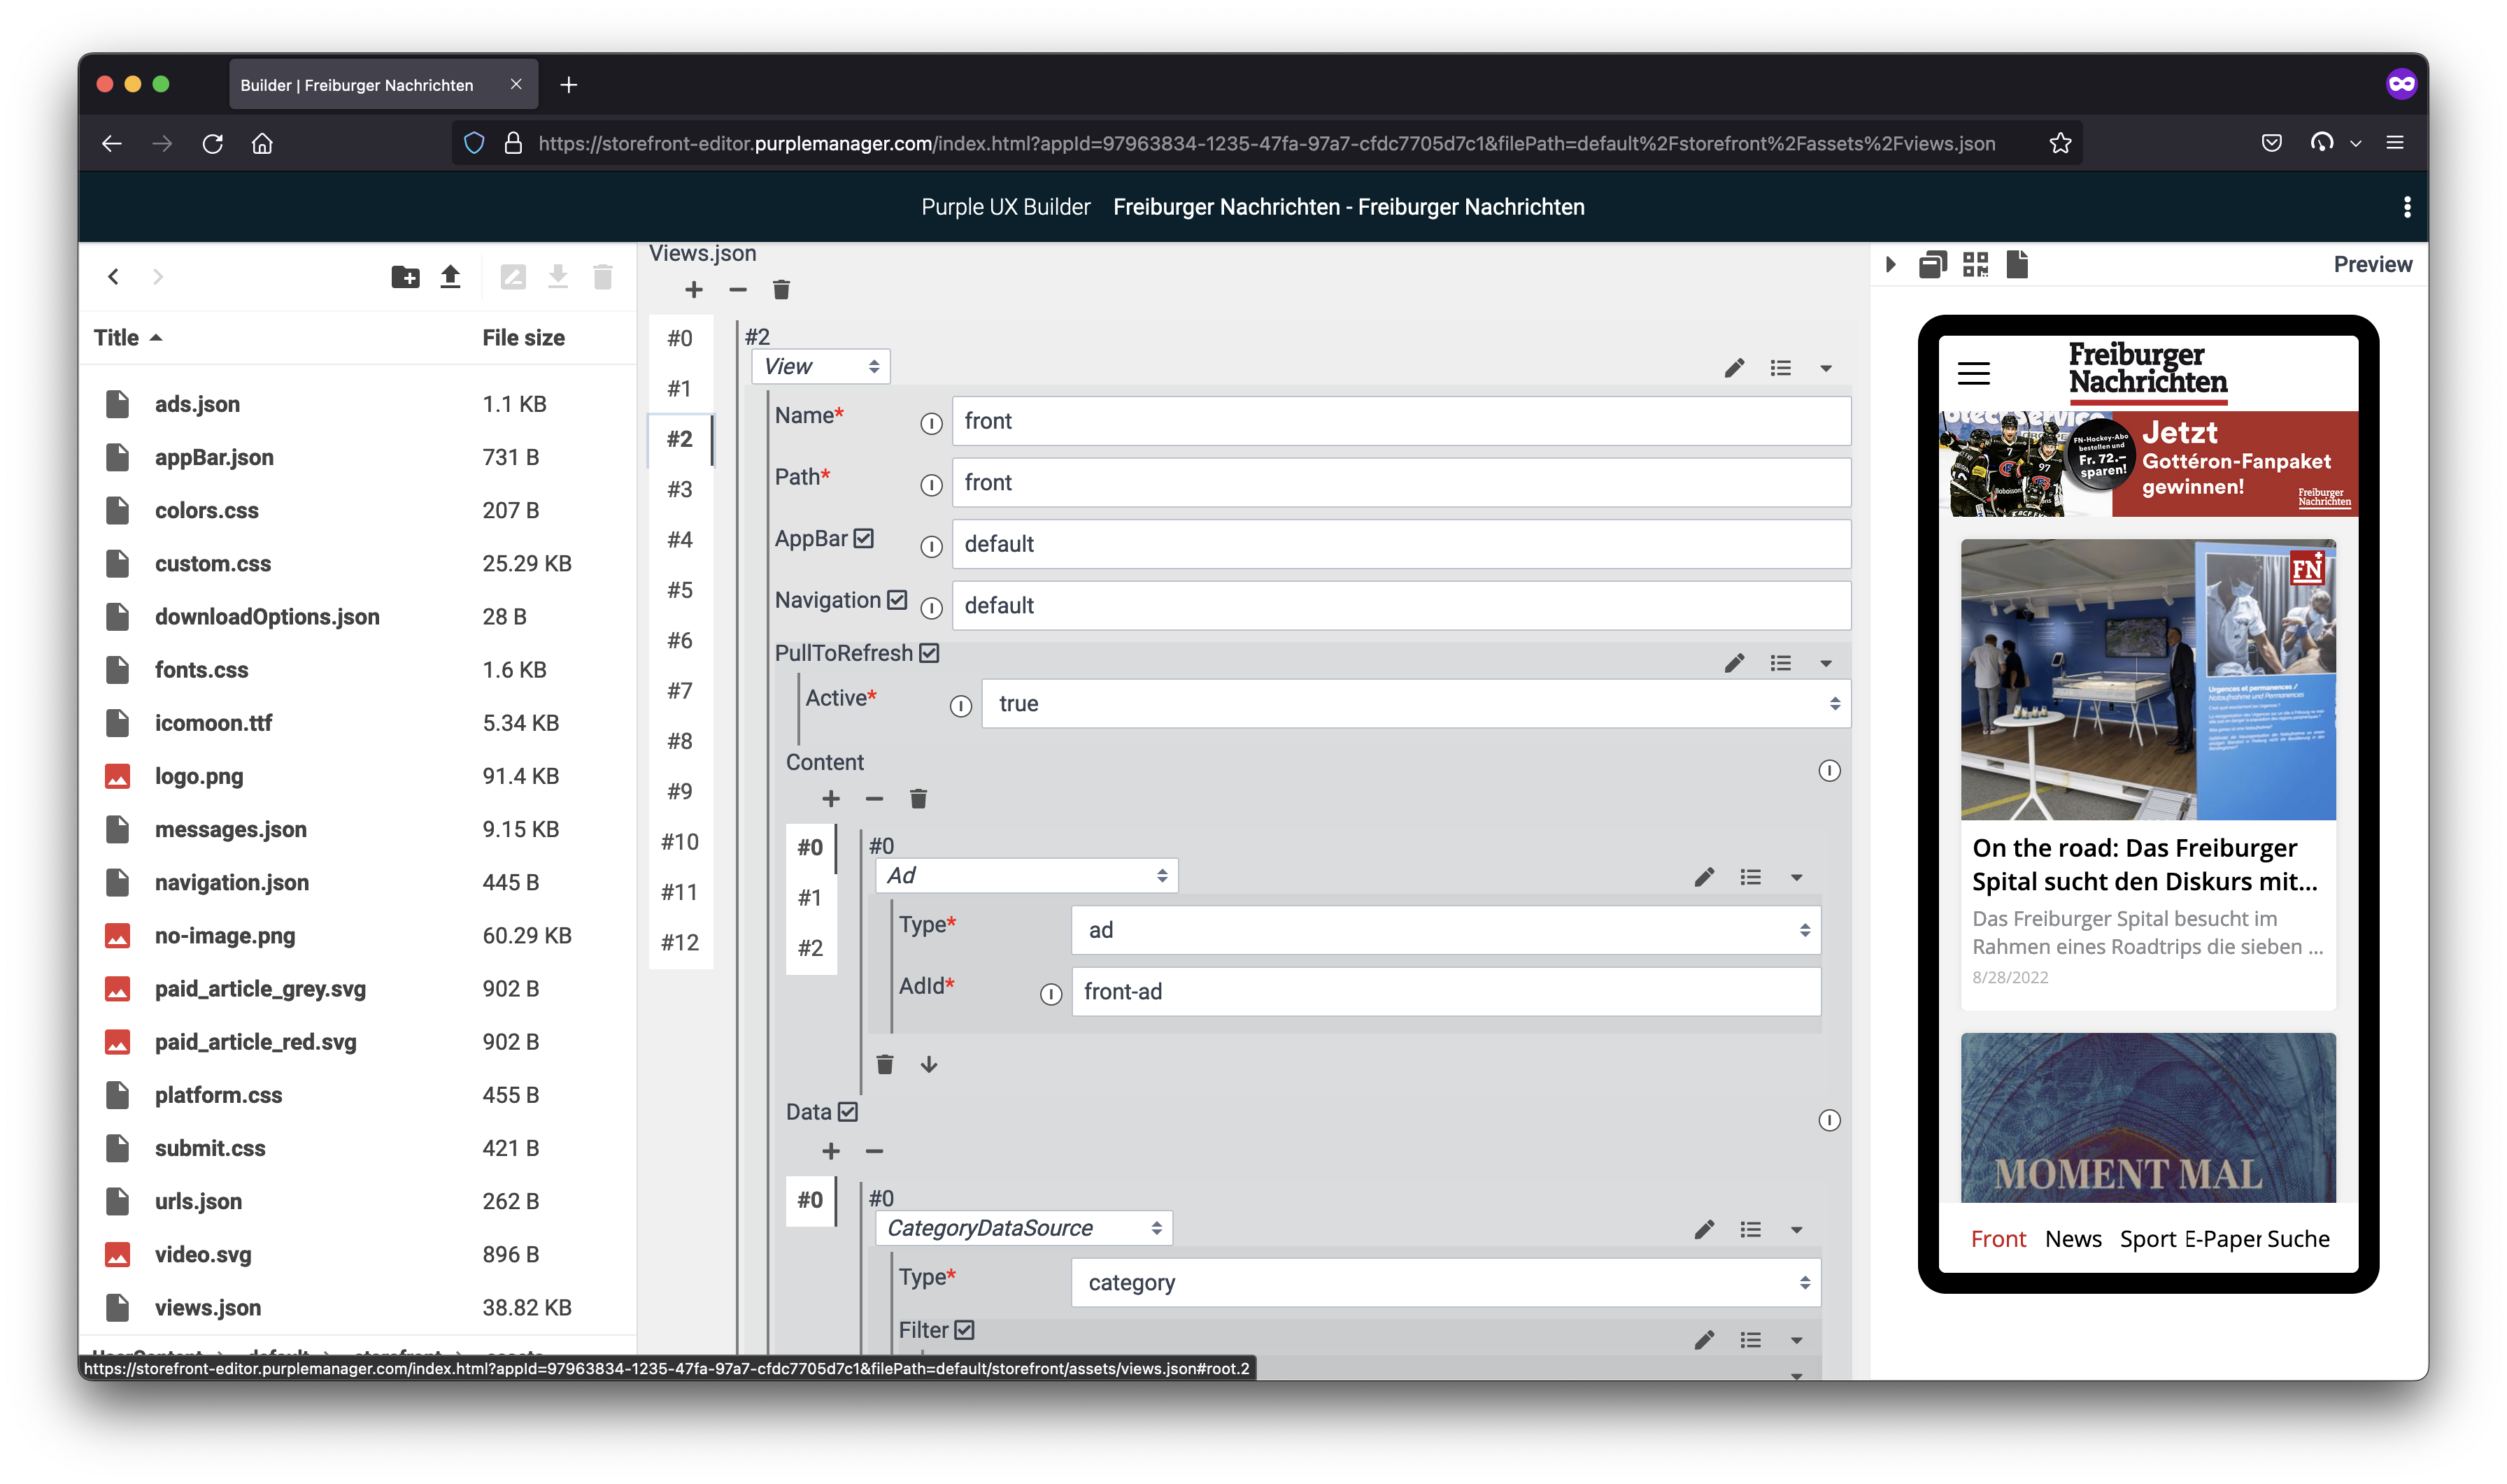
\includegraphics[width=\textwidth]{pics/current_editor.png}
An example of the current editor UI

%************************************************************************
\subsection{Goal}
\label{subsec:goal}
% Gap you want to close with your research.
% Goal of your work.
% Your research question.
% List the main research question(s) you want to answer.
% Explain whether your research will provide a definitive answer or simply contribute towards an answer
%************************************************************************
The goal is to give the diffrent identified possible user groups an editor
which enables them to work more productive, make less errors and get more interactive feedback from the system,
so that there is less support needed by other entities like the framework developers.


This includes evaluating diffrent HCI methods to evaluate the current state as well as the diffrent needs of the users,
and then using an agile development process to build an web based editor for the Purple Experience framework.
The core of this will be an editor to edit the JSON files describing the App's UI, respecting JSON schema definitions
and fitting the users diffrent knowledge and skill levels.

On a more abstract level, the outcome of the thesis should give insights about integrating an new tool / UI into an existing
production enviroment with many constraints, which methods and approaches worked and maybe also which failed.

The contributions I aim to produce with this bachelor thesis are:

\begin{description}[leftmargin=10em,style=nextline]
  \item[software] an web app and backend that serves and present the editor to clients, possibly contributions to open source libraries if required to fulfill the needs of the editor.
  \item[HCI discoveries] documentation to the diffrent methods and approaches used to gain the insight into the users,
  as well as evaluation of the results of these methods and how effective they proved in the context of changing a component inside a larger ecosystem.
  \item[user base knowledge] better knowledge about what the diffrent user groups of the propsed editor are and can be, as well as their diffrent habits, knowledge levels, common mistakes and more.
\end{description}

